\documentclass[9pt,a4paper]{article}
\usepackage[margin=15mm]{geometry}
\usepackage{graphicx,booktabs,microtype,xcolor,hyperref,enumitem}
\usepackage[T1]{fontenc}
\hypersetup{colorlinks=true,urlcolor=blue!55!black,linkcolor=blue!55!black}
\setlength{\parindent}{0pt}
\setlength{\parskip}{3pt}
\setlist{nosep,leftmargin=4mm}
\pagestyle{plain}

\title{\vspace{-12mm}\textbf{EconDID Studio}\\[-1mm]
\large Guided, auditable DID and DDD analysis for applied researchers}
\author{Student: \rule{32mm}{0.4pt} \quad Student ID: \rule{28mm}{0.4pt}\\
Repository: \url{https://github.com/panzehui-gh/econ-did-studio}}
\date{August 2026}

\begin{document}
\maketitle
\vspace{-6mm}

\section*{Purpose and user workflow}
EconDID Studio reduces the repeated programming work between a research design
and an estimable difference-in-differences (DID) or triple-differences (DDD)
model. A researcher uploads a CSV, TSV, or Excel file, selects the closest model
preset, confirms the meaning and positive direction of variables, optionally
adds controls/fixed effects, and downloads a reproducibility bundle. The main
interface is a Streamlit web app, while a command-line interface supports batch
and scripted use. The current scope contains basic 2$\times$2 DID, panel DID with
entity/time fixed effects, custom-fixed-effect DID, and DDD.

Automation does not replace identification. The interface explicitly warns that
causal interpretation requires assumptions such as parallel trends and that its
trend plot is descriptive. Ambiguous two-category labels are never silently
assigned to treatment or control.

\section*{Implementation and design choices}
The pipeline is non-destructive and records every operation: label
normalization, empty/duplicate removal, missing-marker standardization, and
conservative numeric/date conversion. An explainable heuristic ranks candidate
columns for outcome, treatment, post, entity, time, and subgroup. It combines
multilingual name aliases, fuzzy similarity, data type, cardinality, and optional
plain-language descriptions. The user sees confidence, reasons, alternatives,
and confirms the final mapping.

Models are built with statsmodels formulas. HC1 covariance is the default;
cluster-robust covariance is available and is selected automatically by entity
for the two-way fixed-effect preset. Pre-estimation checks require all four DID
cells (or eight DDD cells), exactly two indicator values, complete estimable
observations, and the required panel identifiers. The export ZIP contains the
exact analysis data, coefficient table, formula/coding metadata, diagnostics,
full statsmodels summary, and observed-trend figure. The package also provides
synthetic data generators, a CLI, unit tests, MIT license, and GitHub Actions CI.

\newpage
\section*{Objective validation}
Synthetic balanced panels were generated from known data-generating processes.
Twenty independent seeds were used for each estimator (40 fits total), with
entity-clustered standard errors and entity/time fixed effects where appropriate.
For DID, the true effect was 2.0: mean estimate 1.9988, bias $-0.0012$, RMSE
0.0904, and 95\% interval coverage 0.95. For DDD, the true effect was 1.5: mean
estimate 1.4512, bias $-0.0488$, RMSE 0.1496, and coverage 1.00. The automated
test suite also checks dirty-data conversion, multilingual role mapping,
indicator-direction safeguards, missing-cell rejection, input immutability,
result export, and a headless run of the web app.

\begin{center}
\begin{minipage}{0.82\linewidth}
\centering
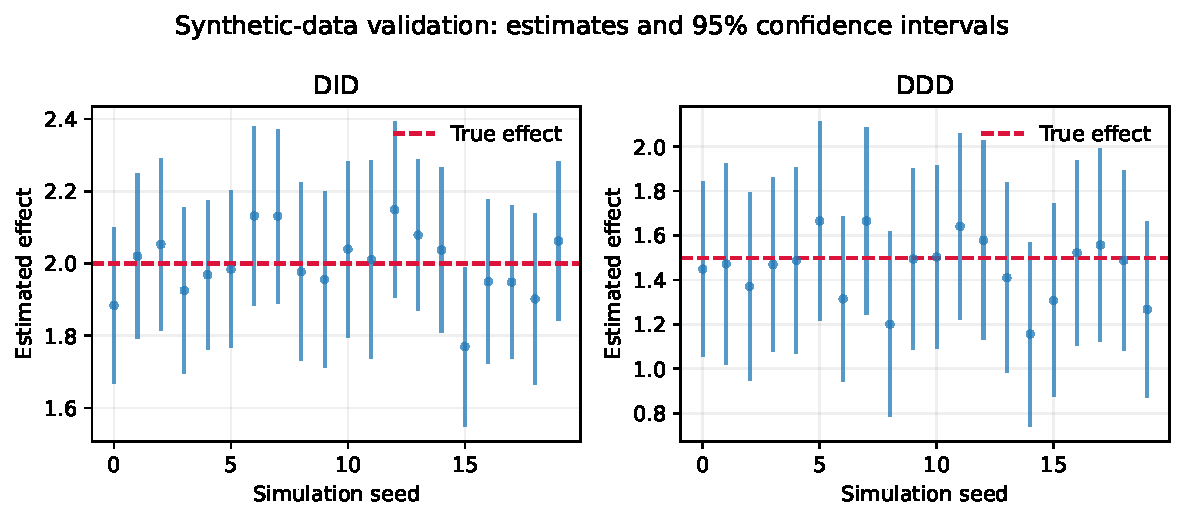
\includegraphics[width=\linewidth]{../docs/validation/validation_results.pdf}
\vspace{-2mm}

{\small Figure 1: Estimates and 95\% confidence intervals across synthetic seeds;
the dashed line is the known effect.}
\end{minipage}
\end{center}

\section*{AI use and reproducibility}
OpenAI Codex (GPT-5) was used to help translate requirements into a software
architecture, draft implementation/tests/documentation, and diagnose test
failures. I reviewed the generated code through executable unit tests and
known-effect simulations rather than accepting output by inspection. No secret,
personal, or externally supplied research data is included. Dependency versions
are declared in \texttt{pyproject.toml}; installation, launch, CLI examples, test
commands, limitations, and CI status are documented in the repository README.

\end{document}
